% !TeX spellcheck = en_GB
\begin{figure}[h]
	%	\centering
	\begin{subfigure}[b]{0.84\textwidth}
		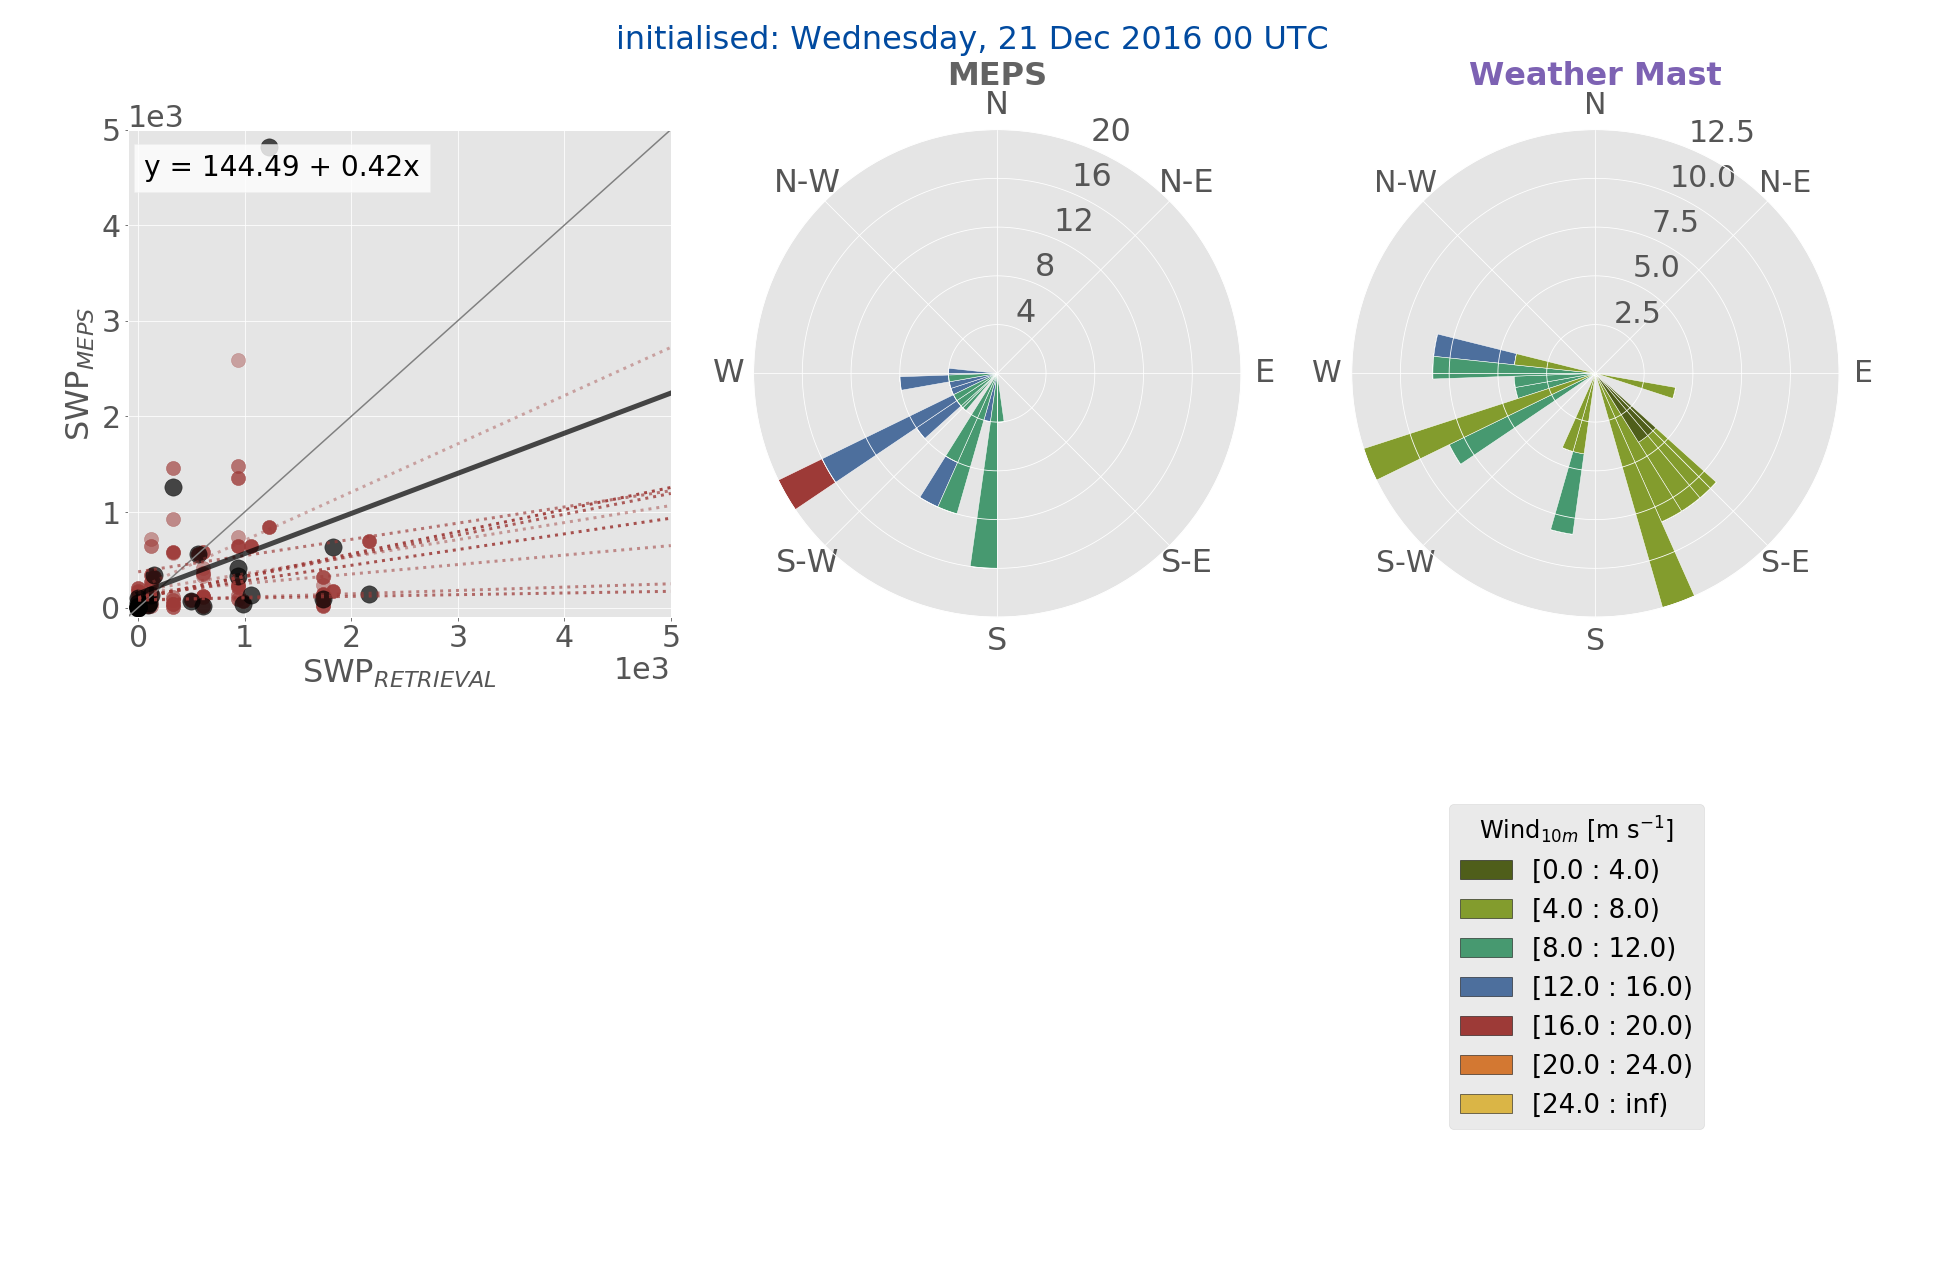
\includegraphics[trim={2.3cm 19.5cm 2.cm .7cm},clip,width=\textwidth]{./fig_windrose/20161221}
		\caption{}\label{fig:wind21}
	\end{subfigure}
	\begin{subfigure}[b]{0.15\textwidth}
		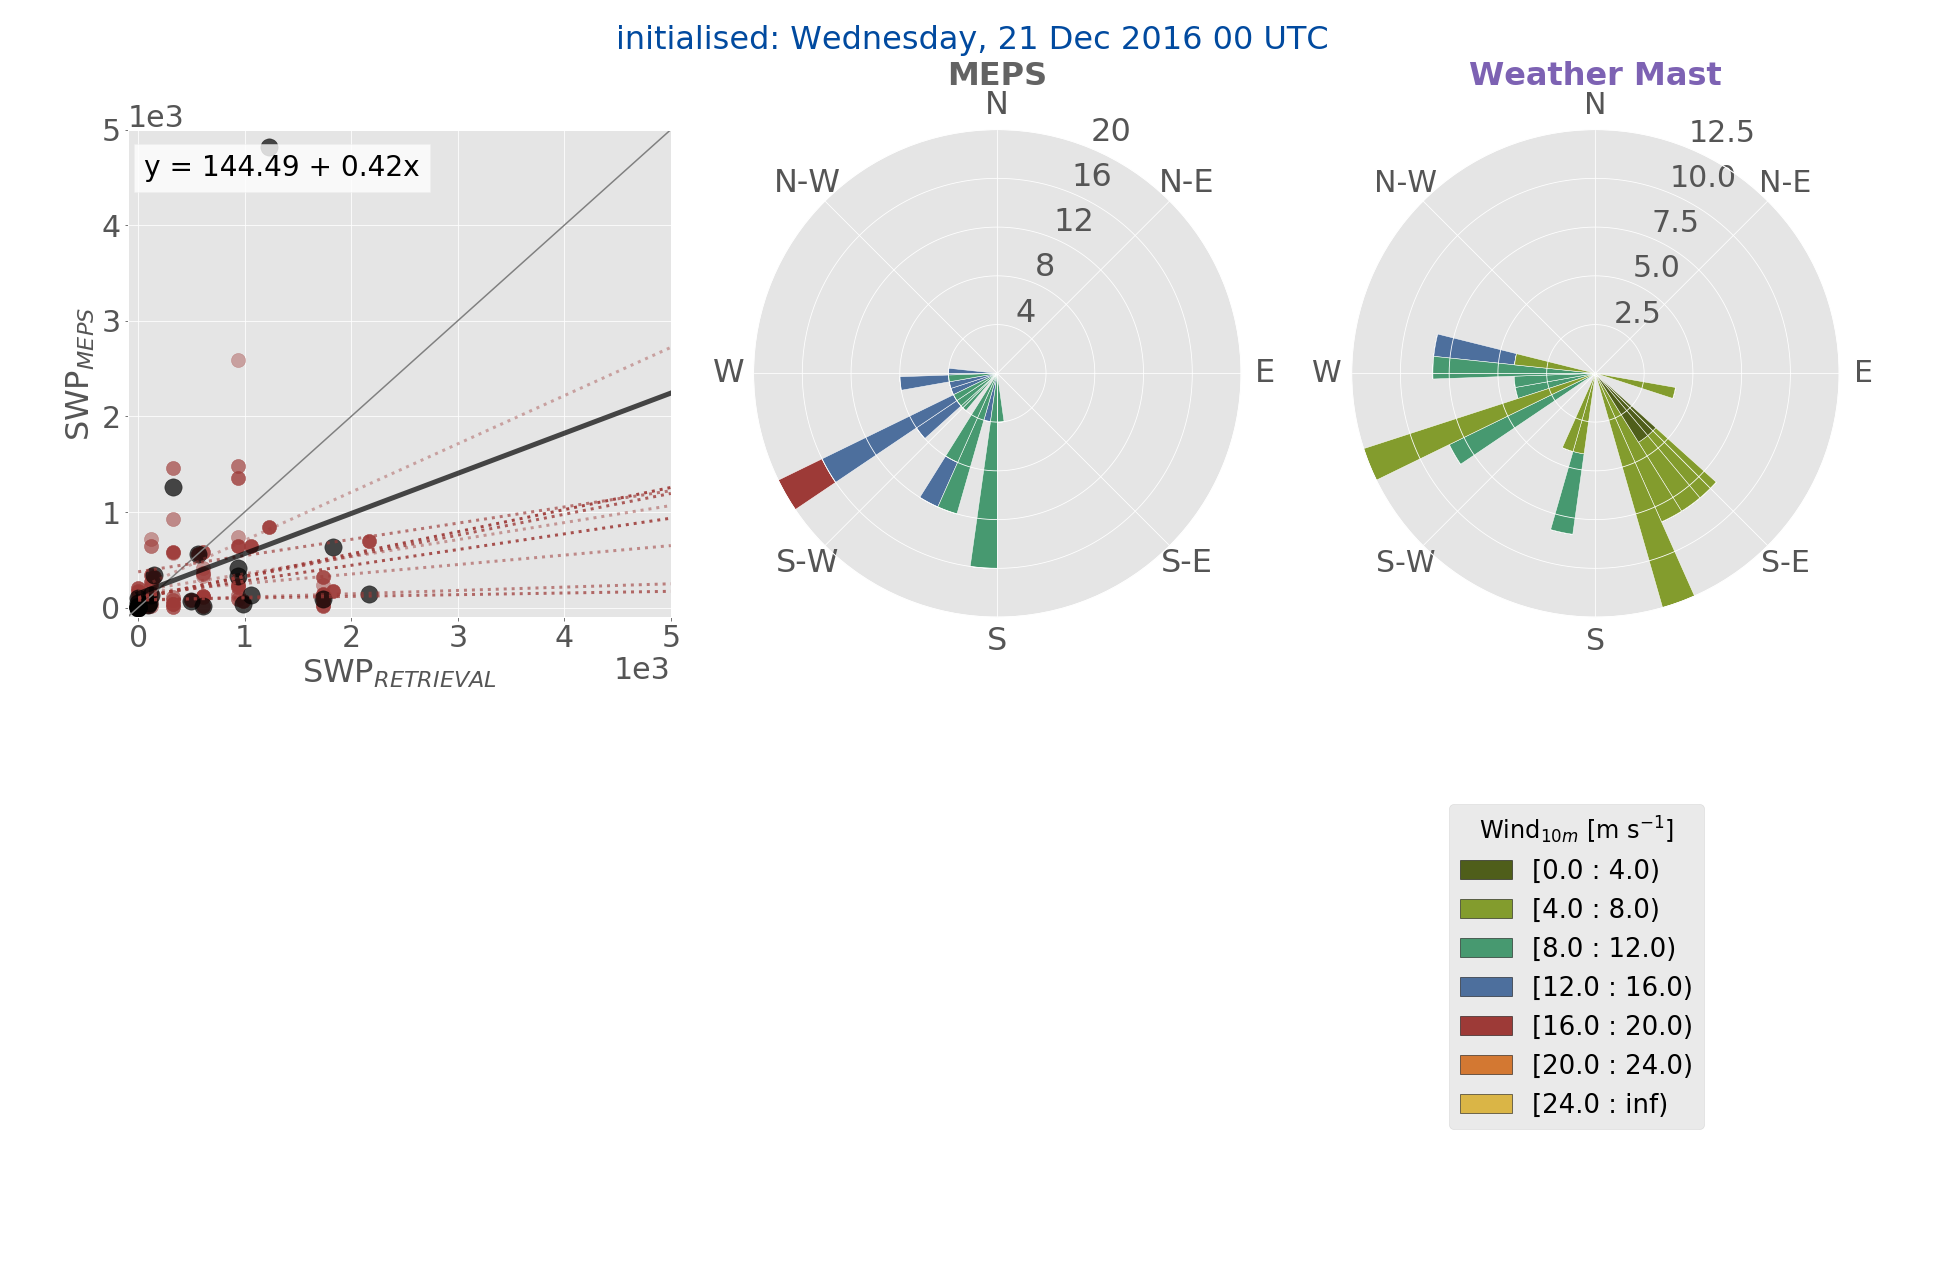
\includegraphics[trim={50.cm 0.cm 8.3cm 28.4cm},clip,width=\textwidth]{./fig_windrose/20161221}
	\end{subfigure}
	\newline
	\begin{subfigure}[b]{0.84\textwidth}
		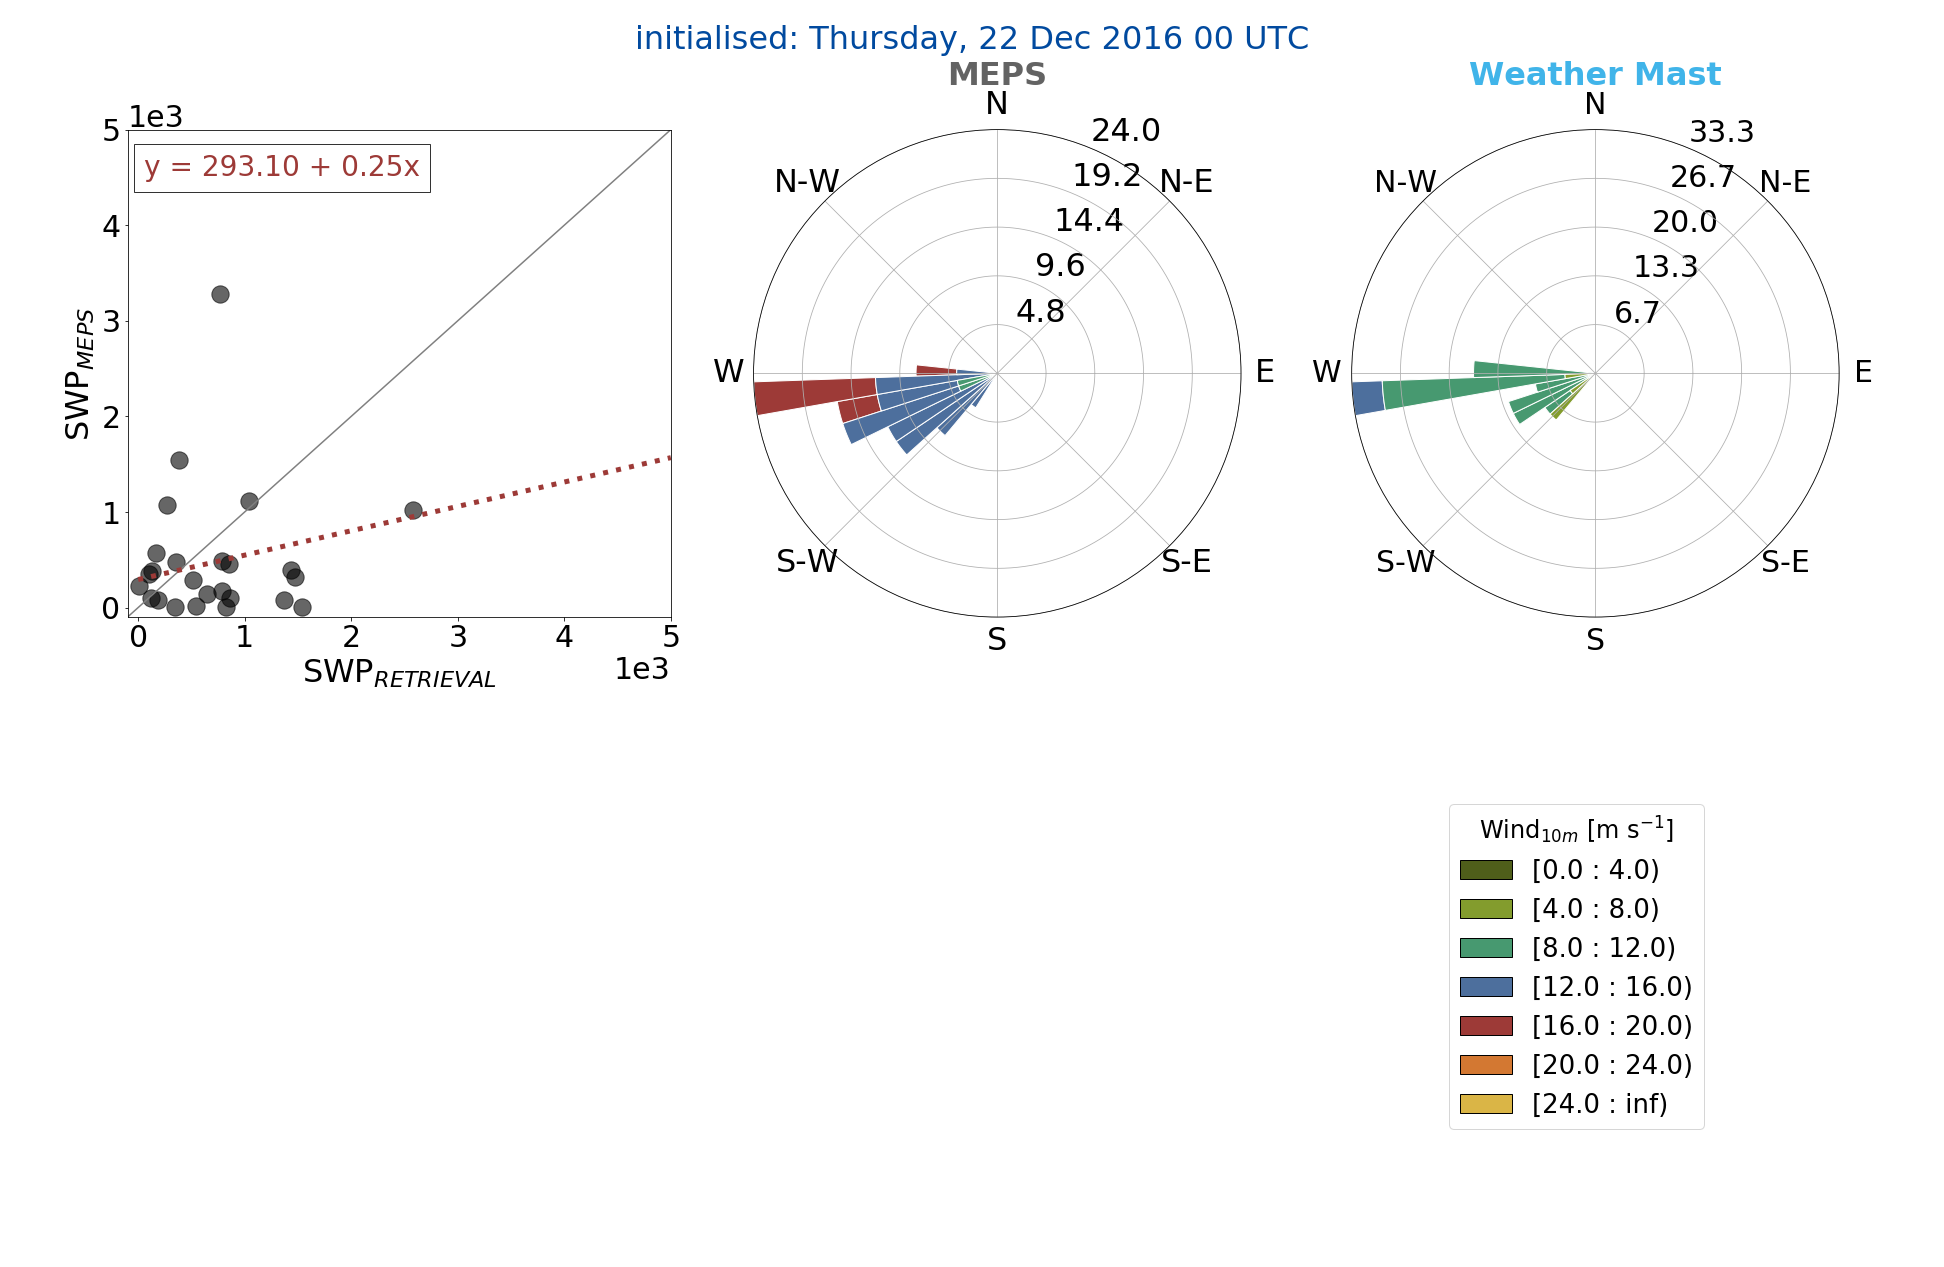
\includegraphics[trim={2.3cm 19.5cm 2.cm .7cm},clip,width=\textwidth]{./fig_windrose/20161222}
		\caption{}\label{fig:wind22}
	\end{subfigure}
	% 	\begin{subfigure}[b]{0.15\textwidth}
	% 		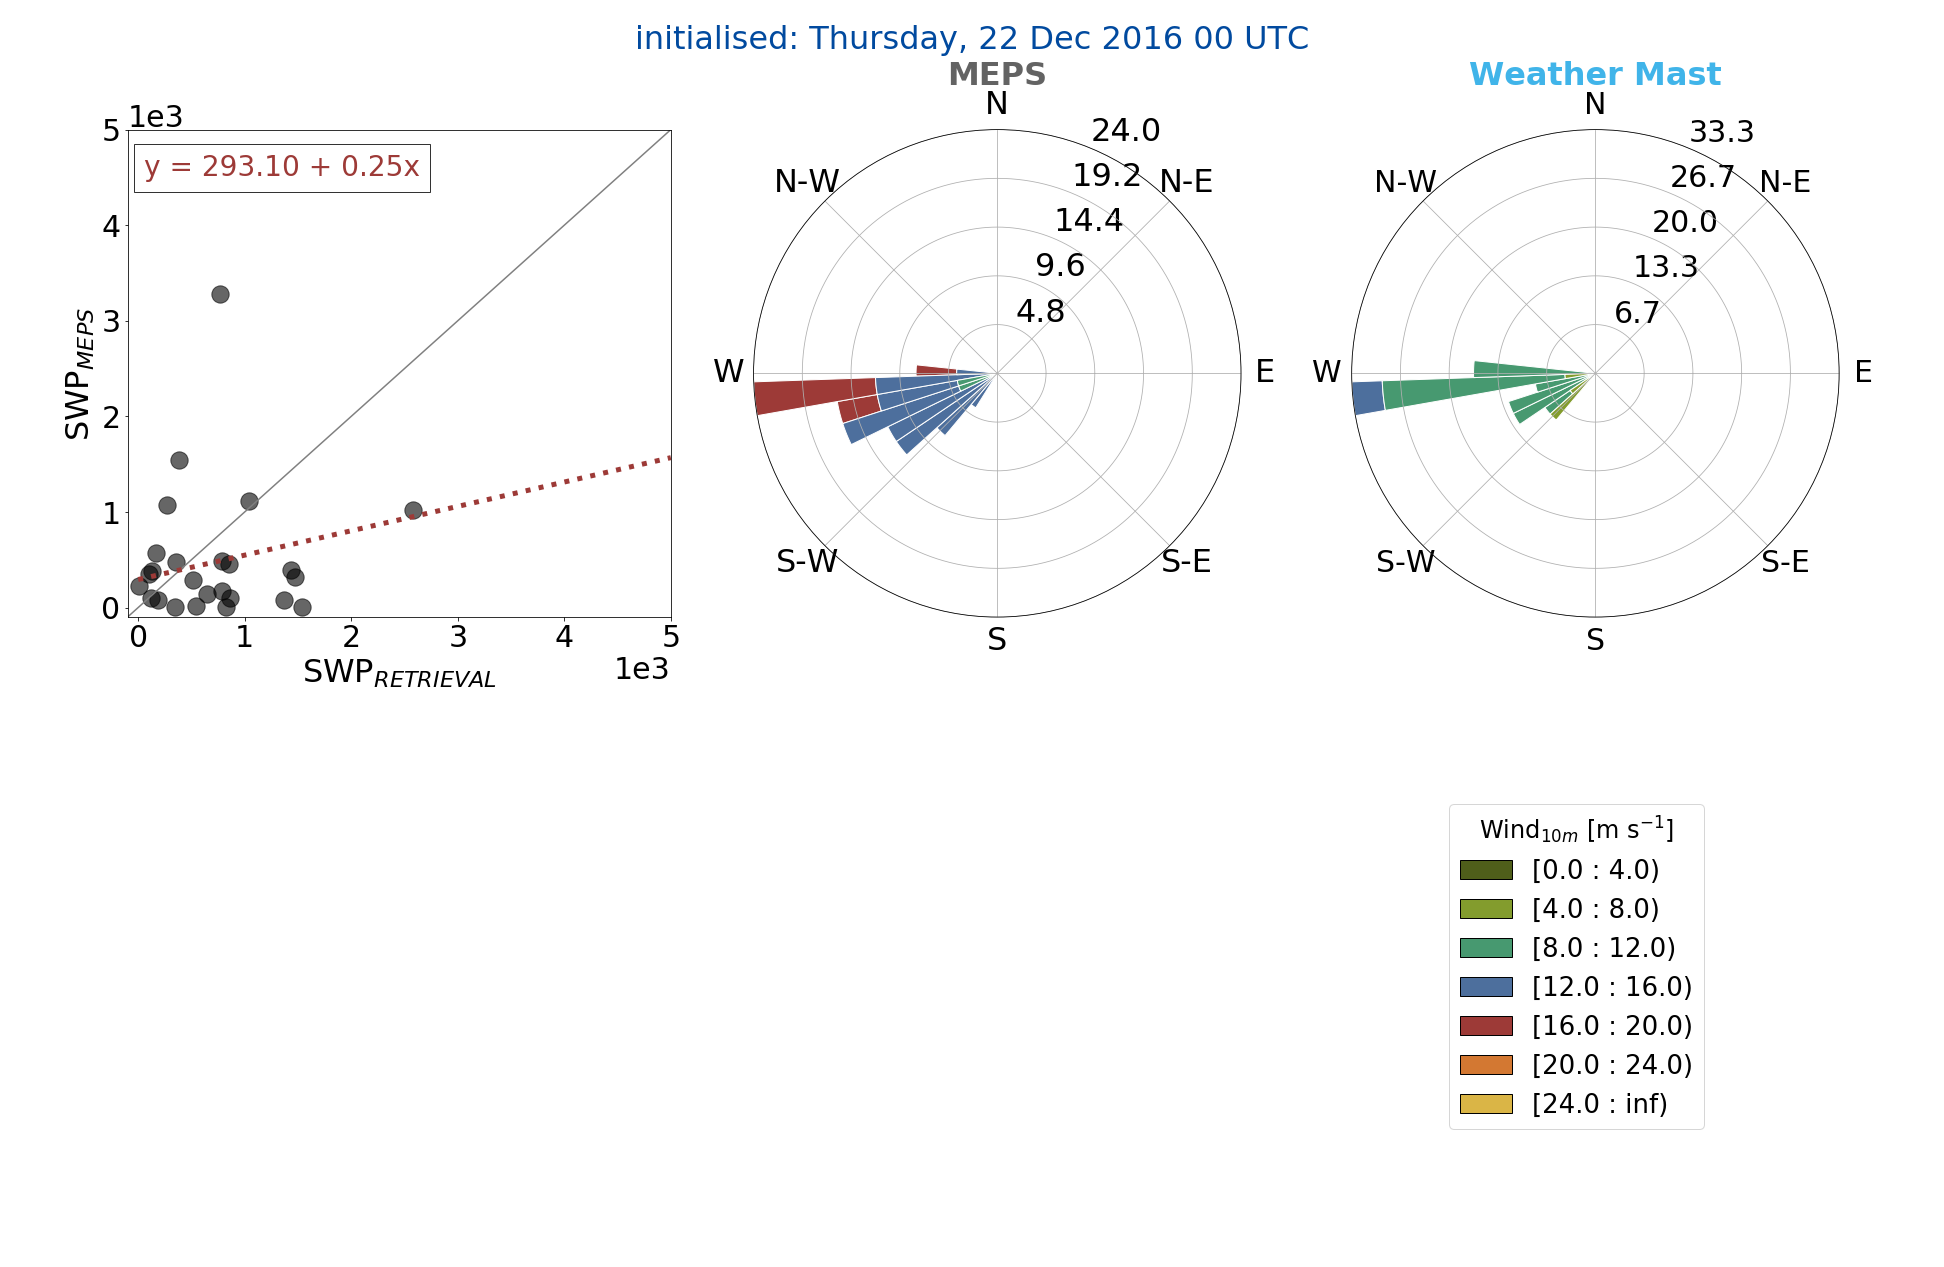
\includegraphics[trim={50.cm 0.cm 8.3cm 28.4cm},clip,width=\textwidth]{./fig_windrose/20161222}
	% 	\end{subfigure}
	\newline
	\begin{subfigure}[b]{0.84\textwidth}
		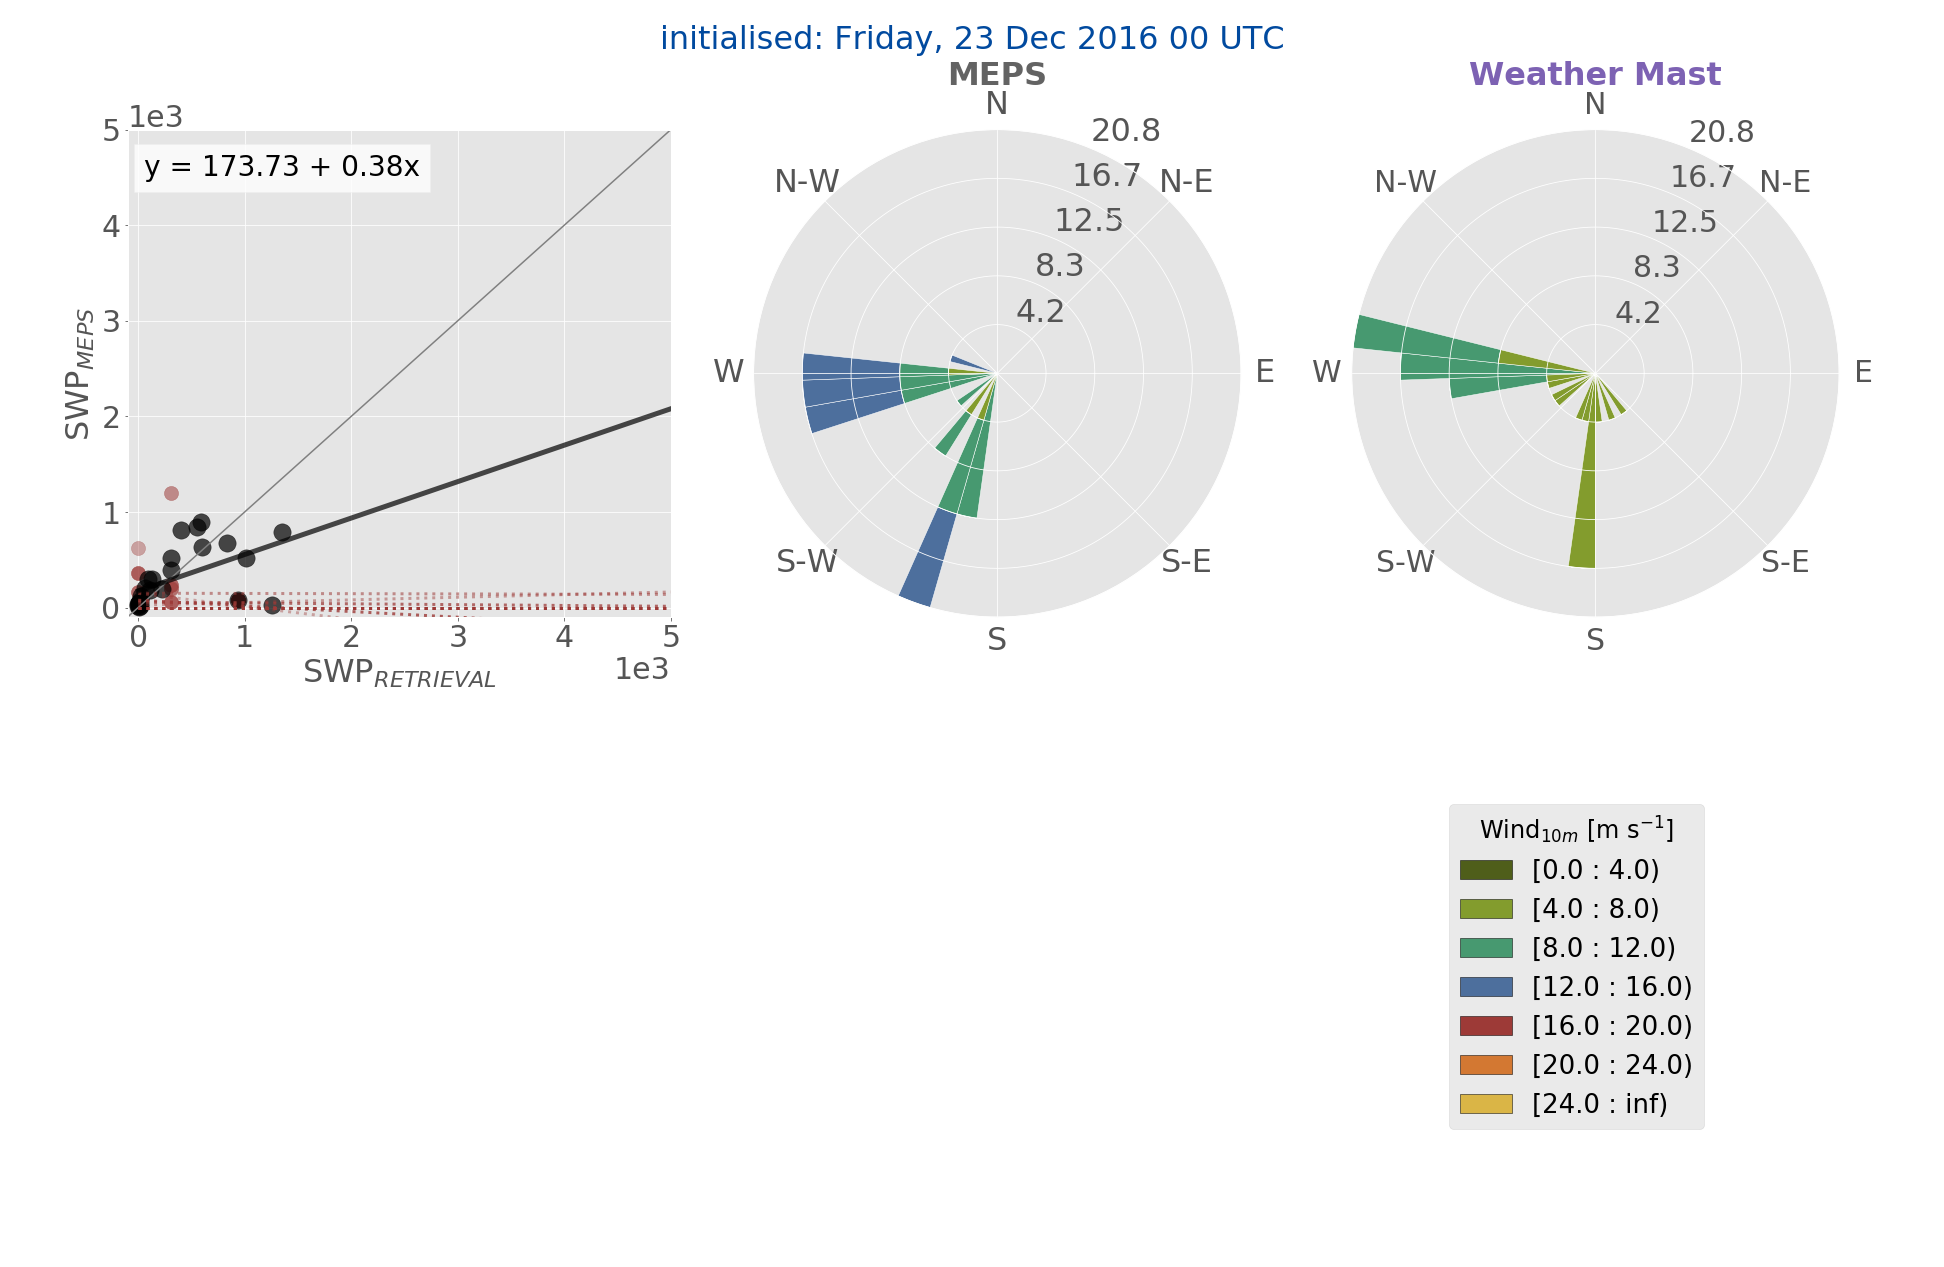
\includegraphics[trim={2.3cm 19.5cm 2.cm .7cm},clip,width=\textwidth]{./fig_windrose/20161223}
		\caption{}\label{fig:wind23}
	\end{subfigure}
	% 	\begin{subfigure}[b]{0.15\textwidth}
	% 		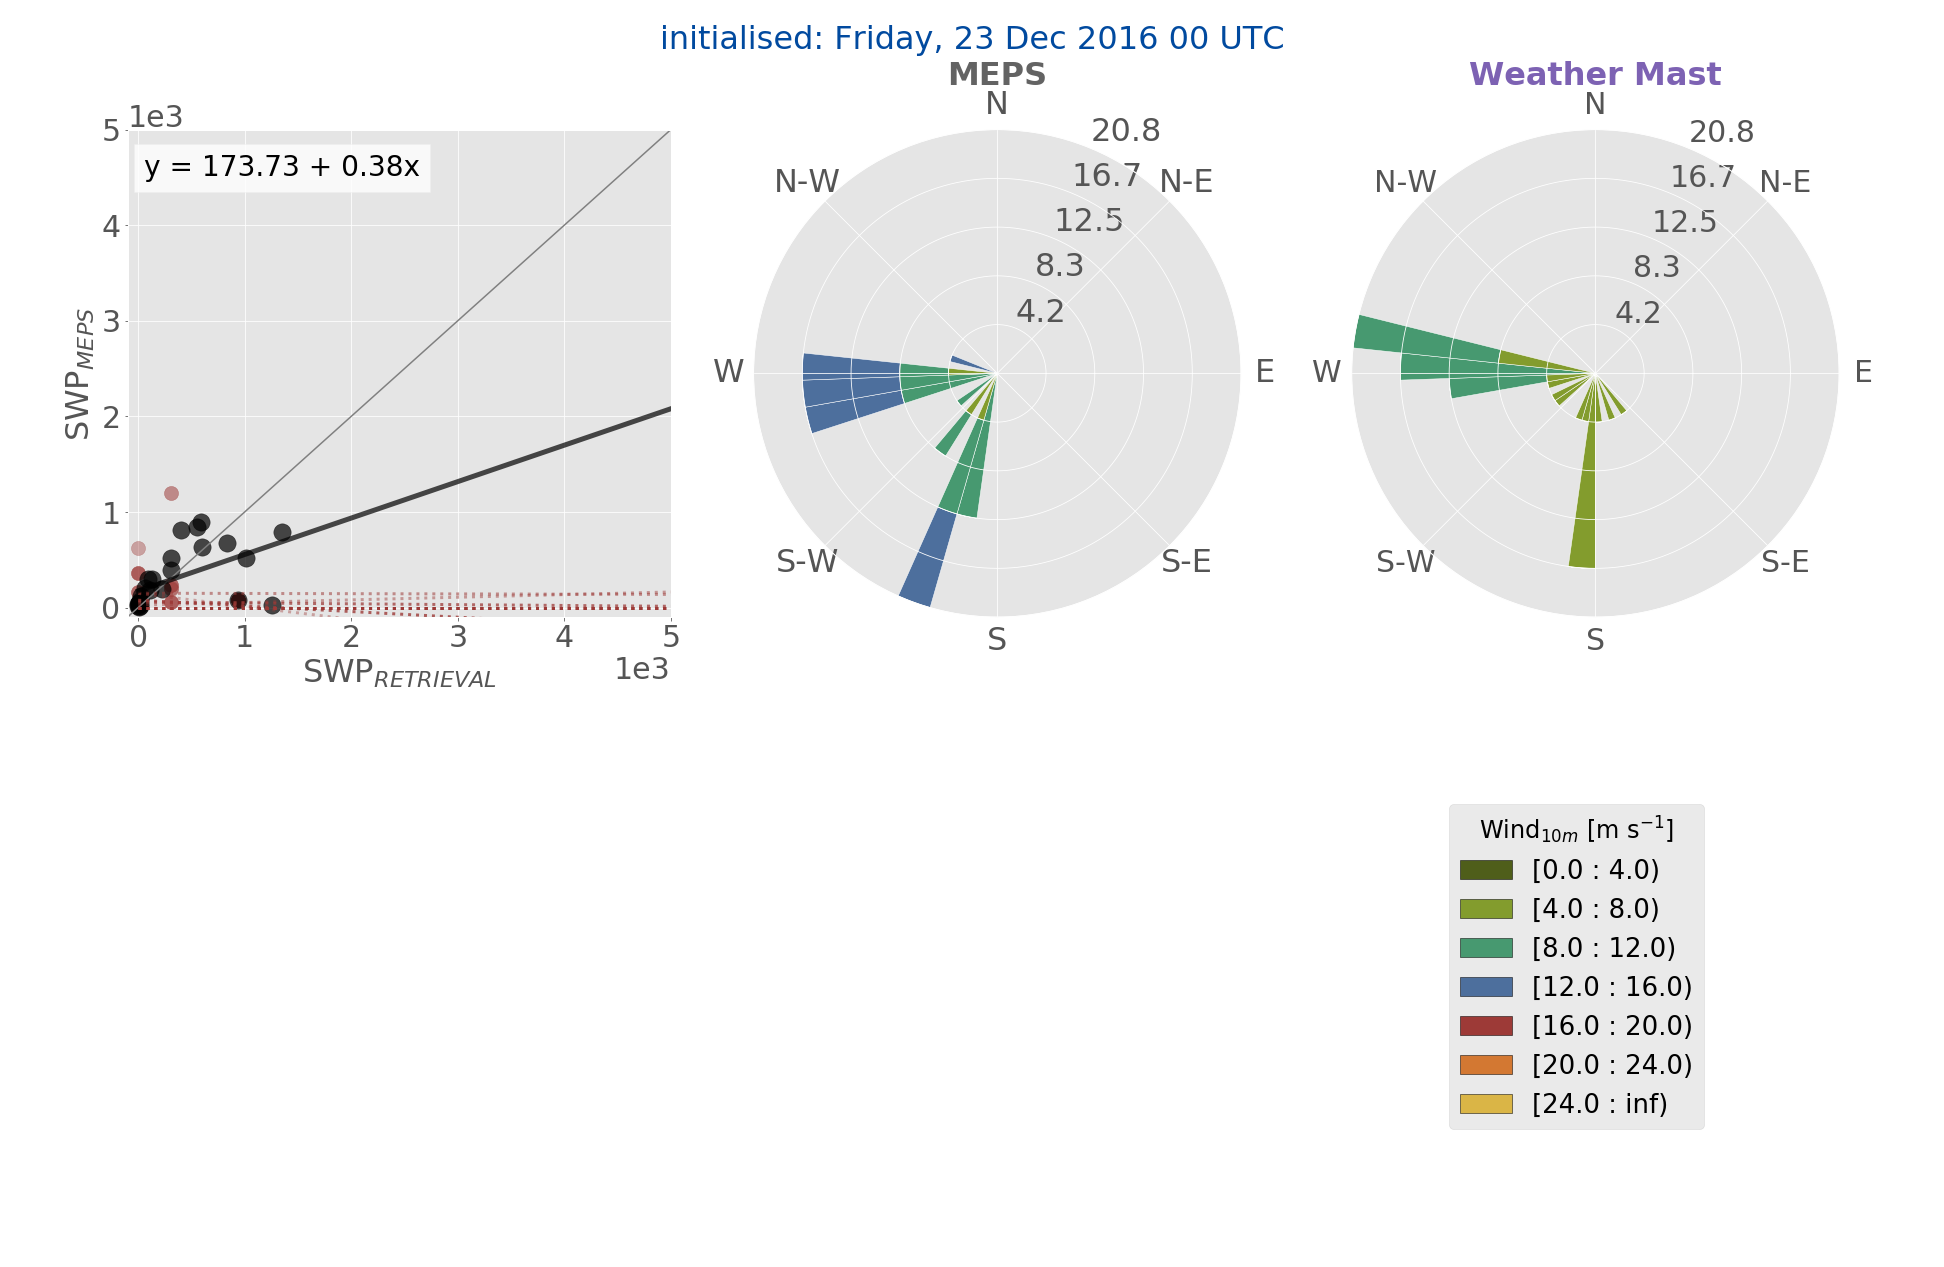
\includegraphics[trim={50.cm 0.cm 8.3cm 28.4cm},clip,width=\textwidth]{./fig_windrose/20161223}
	% 	\end{subfigure}
\end{figure}
%
\begin{figure}\ContinuedFloat
	%	\centering
	\begin{subfigure}[b]{0.84\textwidth}
		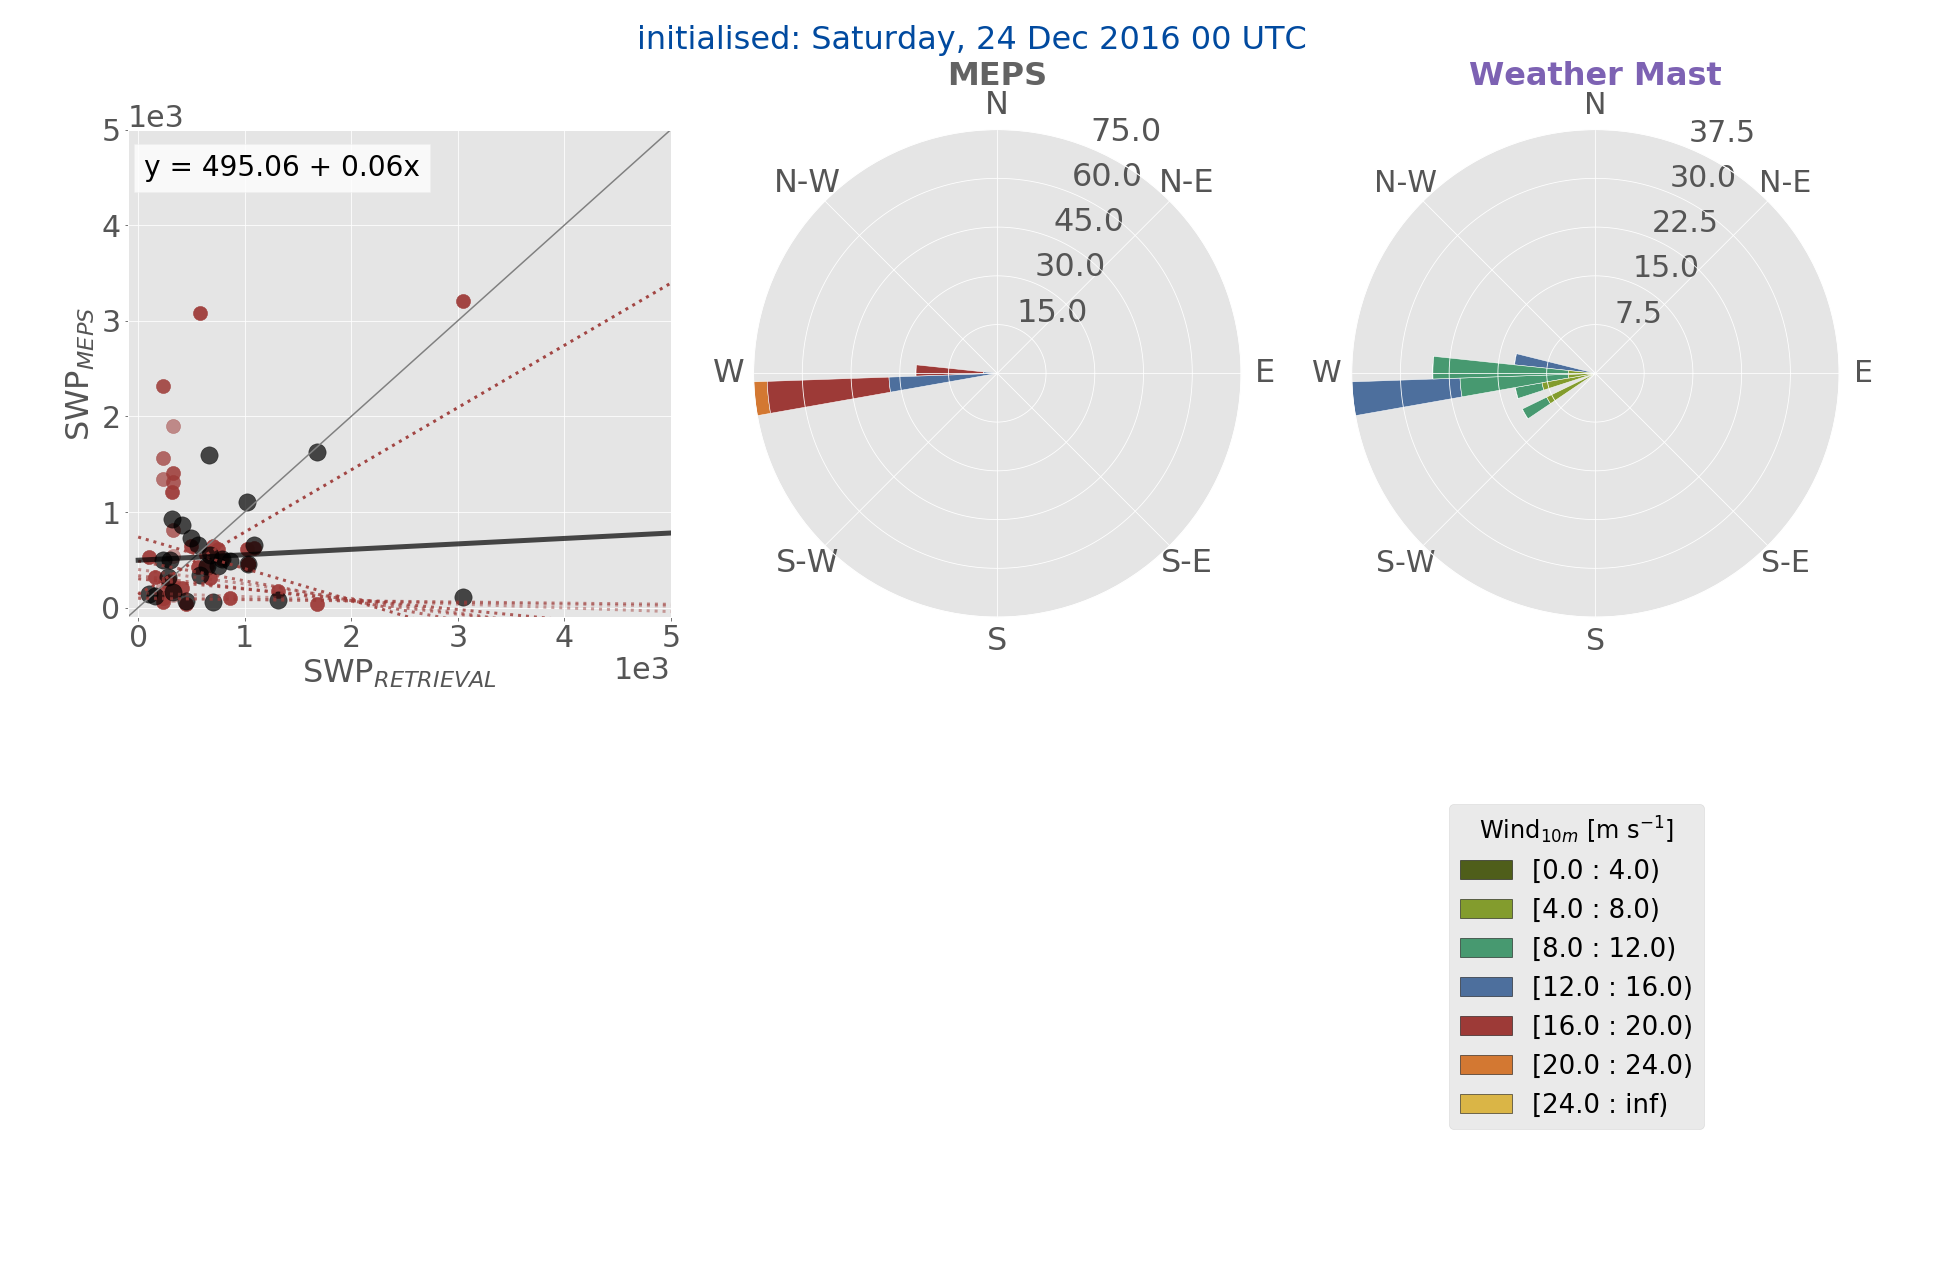
\includegraphics[trim={2.3cm 19.5cm 2.cm .7cm},clip,width=\textwidth]{./fig_windrose/20161224}
		\caption{}\label{fig:wind24}
	\end{subfigure}
	% 	\begin{subfigure}[b]{0.15\textwidth}
	% 		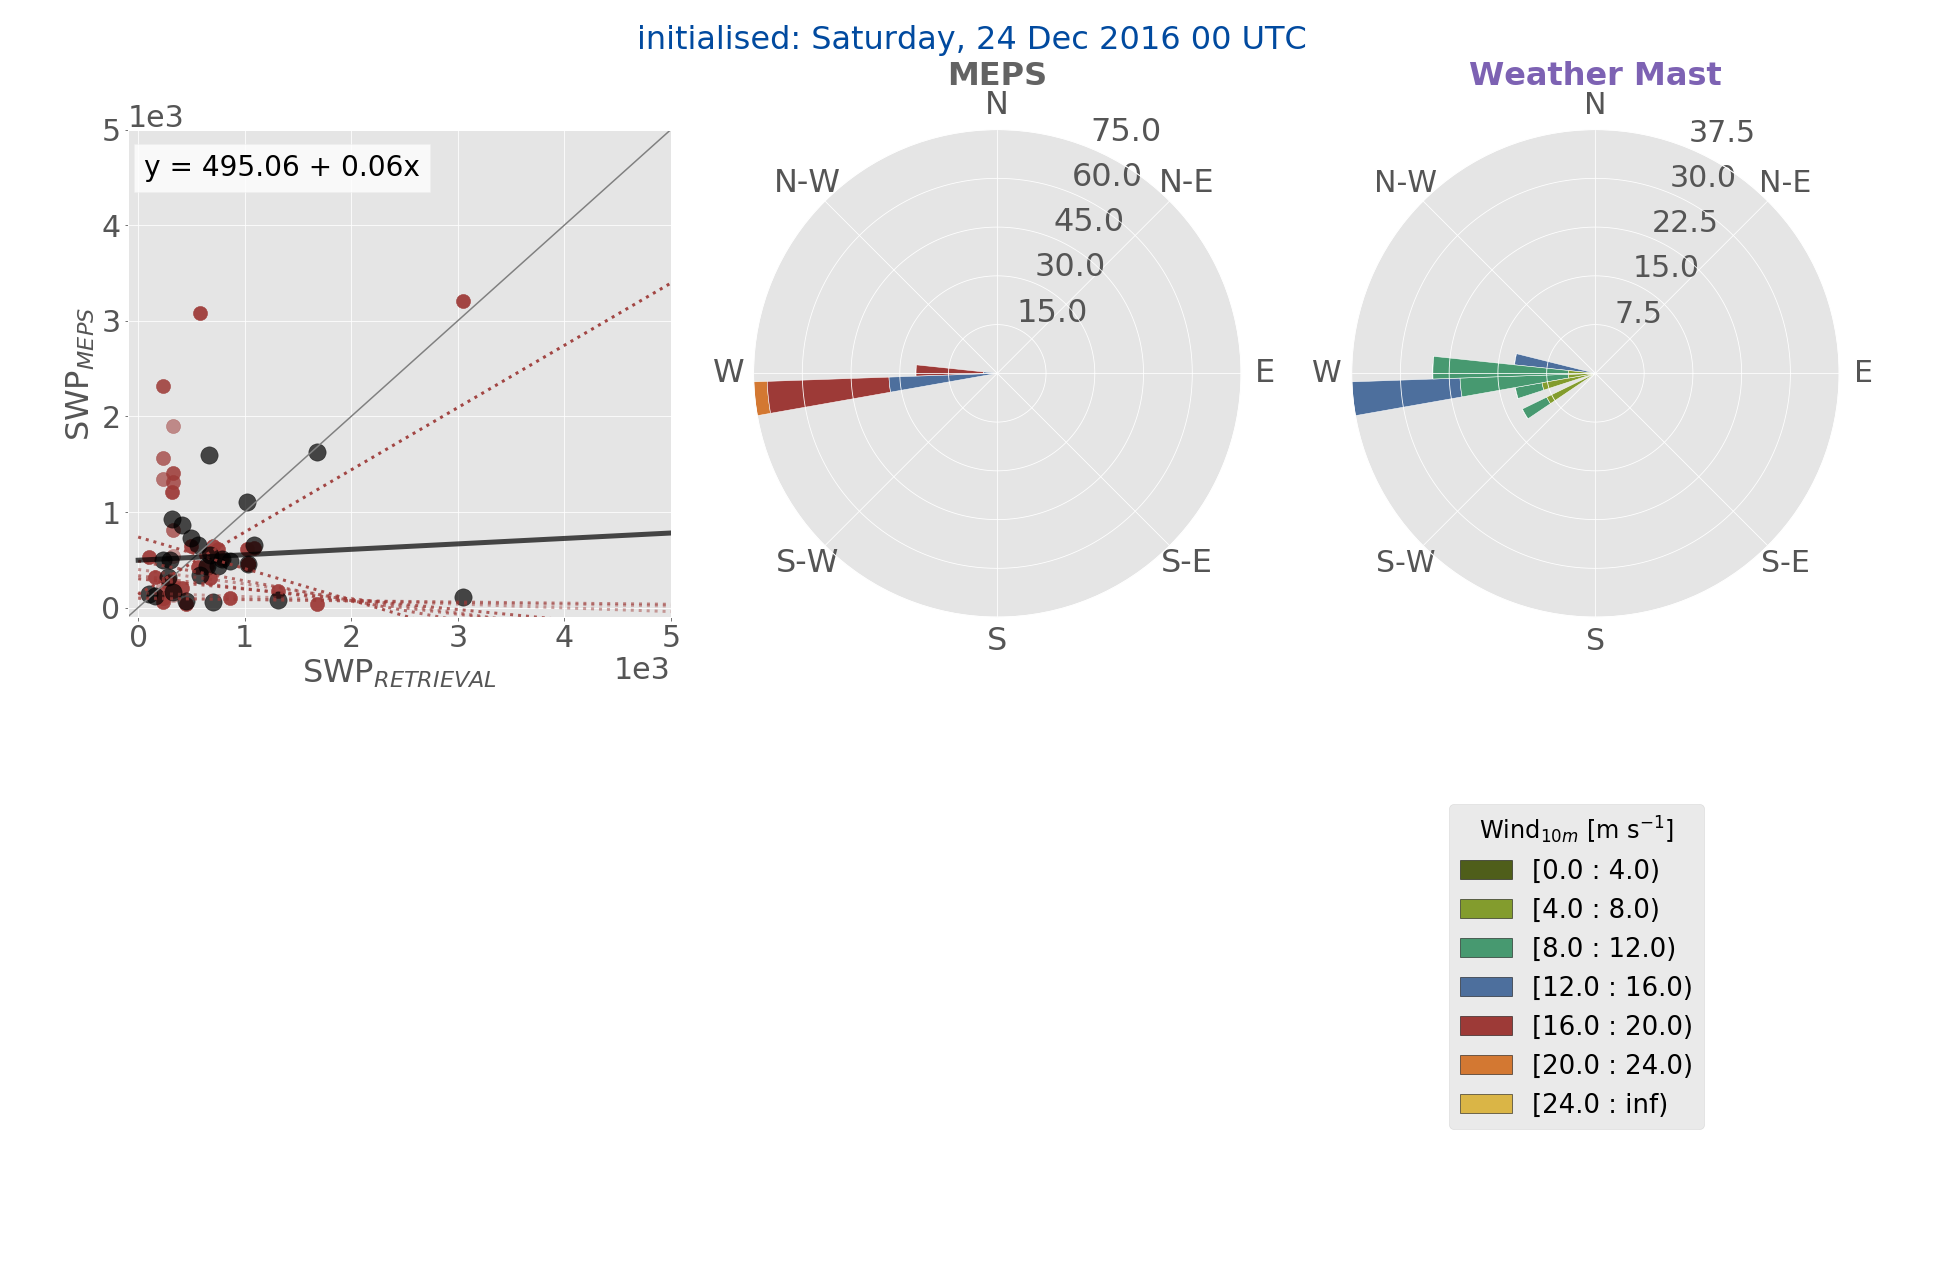
\includegraphics[trim={50.cm 0.cm 8.3cm 28.4cm},clip,width=\textwidth]{./fig_windrose/20161224}
	% 	\end{subfigure}
	\newline
	\centering
	\begin{subfigure}[b]{0.84\textwidth}
		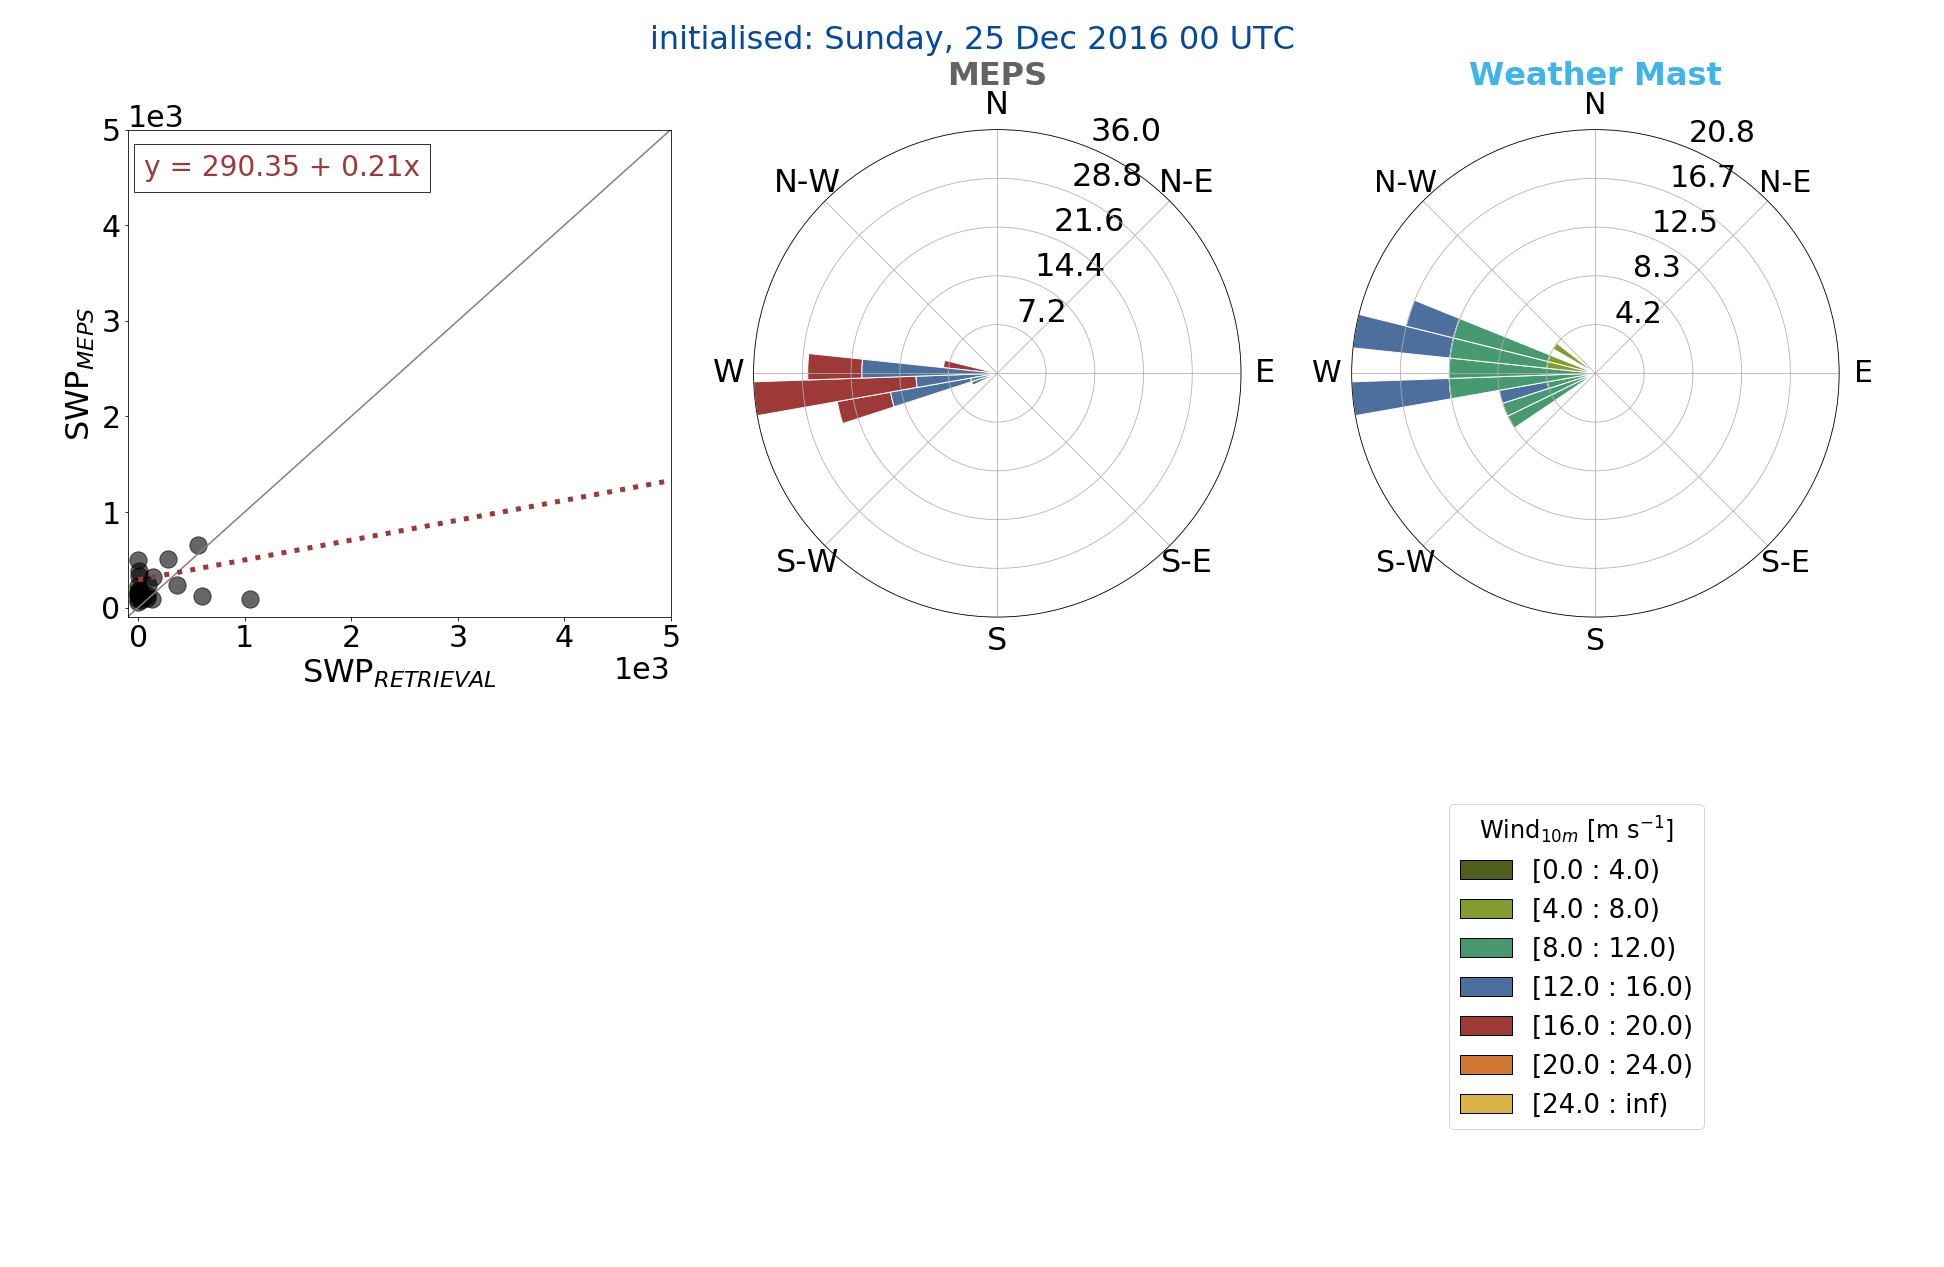
\includegraphics[trim={2.3cm 19.5cm 2.cm .7cm},clip,width=\textwidth]{./fig_windrose/20161225}
		\caption{}\label{fig:wind25}
	\end{subfigure}
	% 	\begin{subfigure}[b]{0.15\textwidth}
	% 		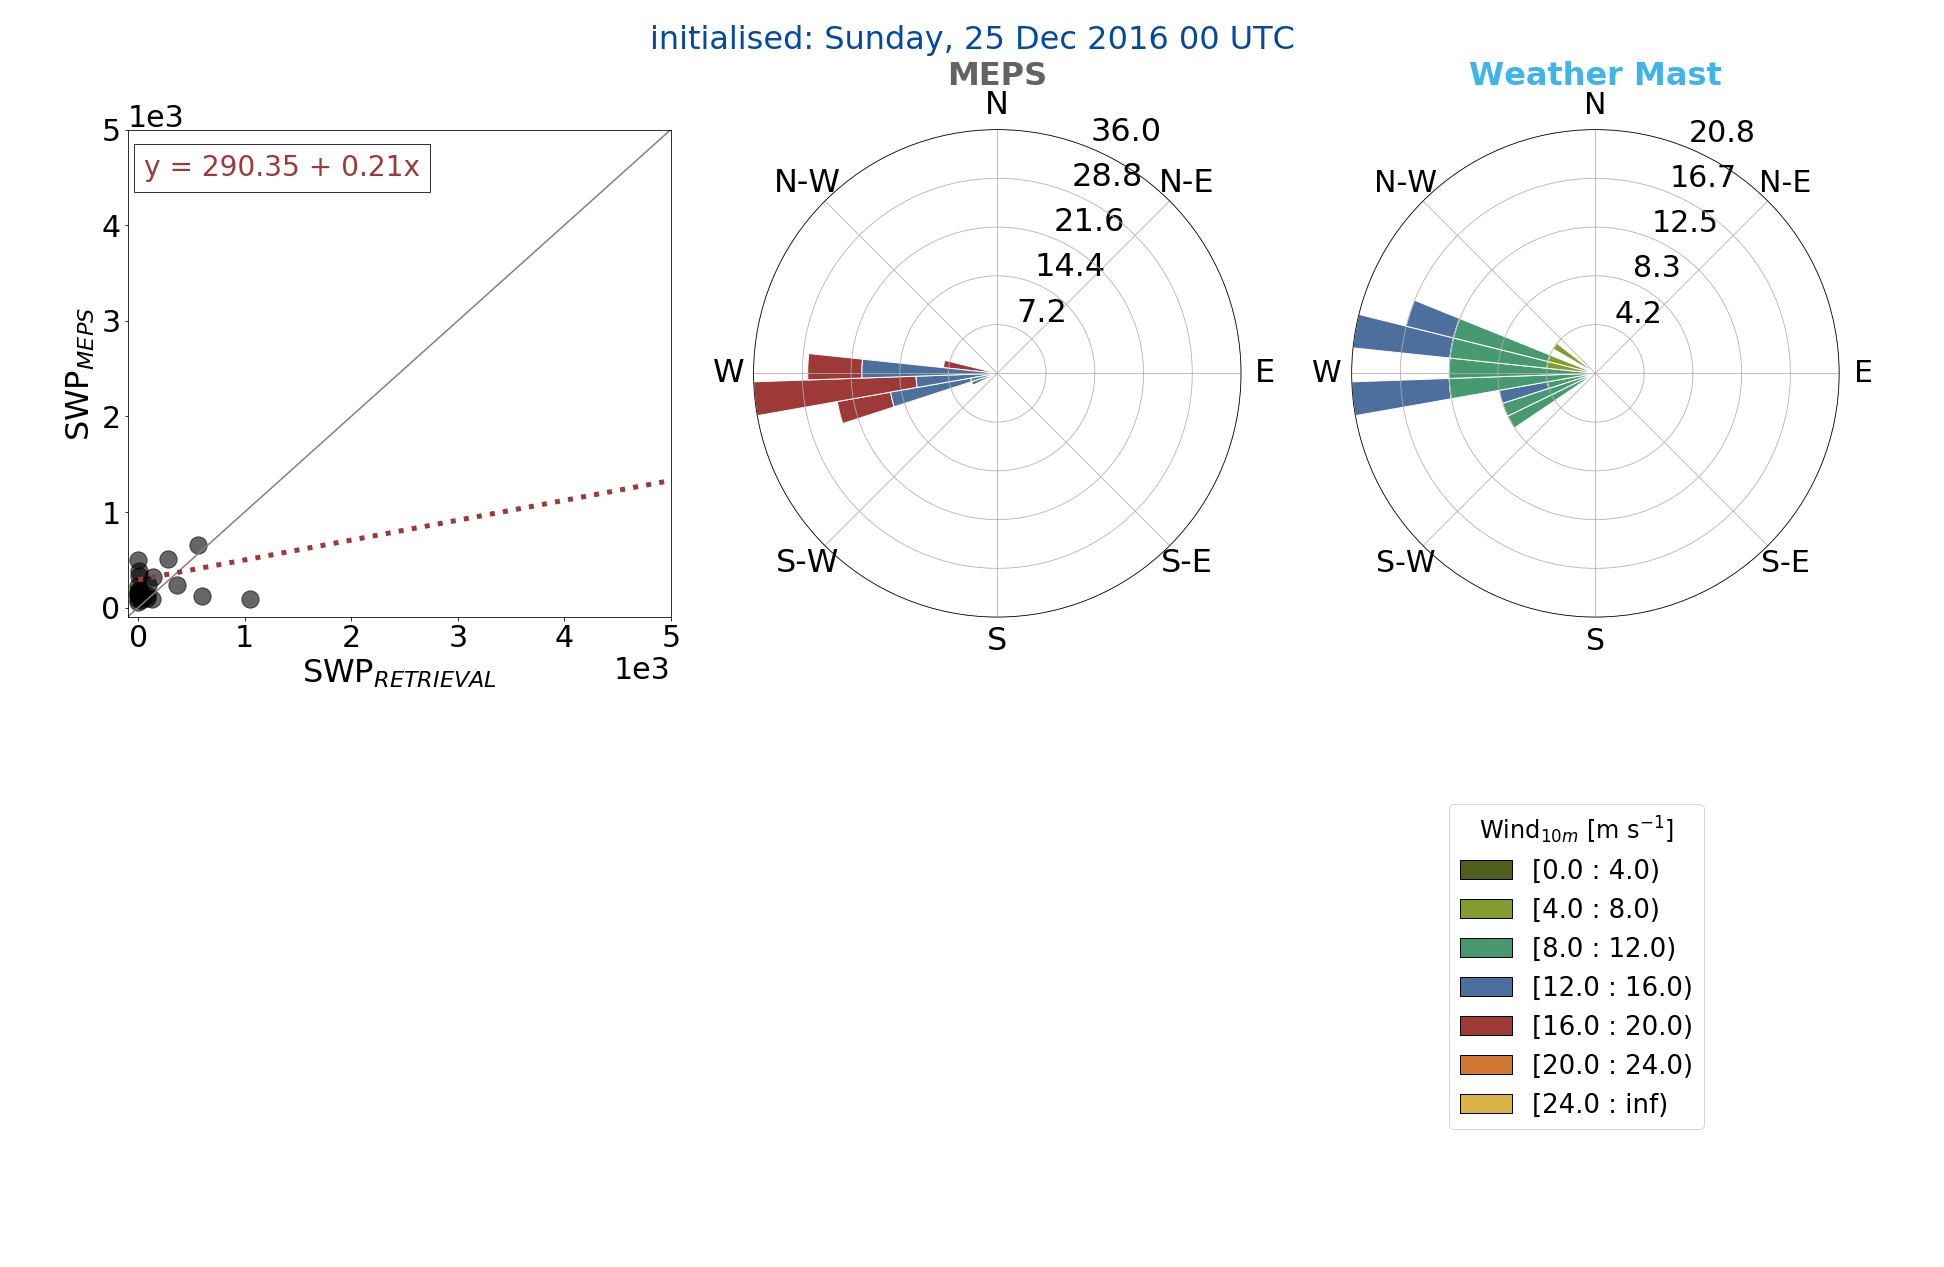
\includegraphics[trim={50.cm 0.cm 8.3cm 28.4cm},clip,width=\textwidth]{./fig_windrose/20161225}
	% 	\end{subfigure}
	\newline
	\begin{subfigure}[b]{0.84\textwidth}
		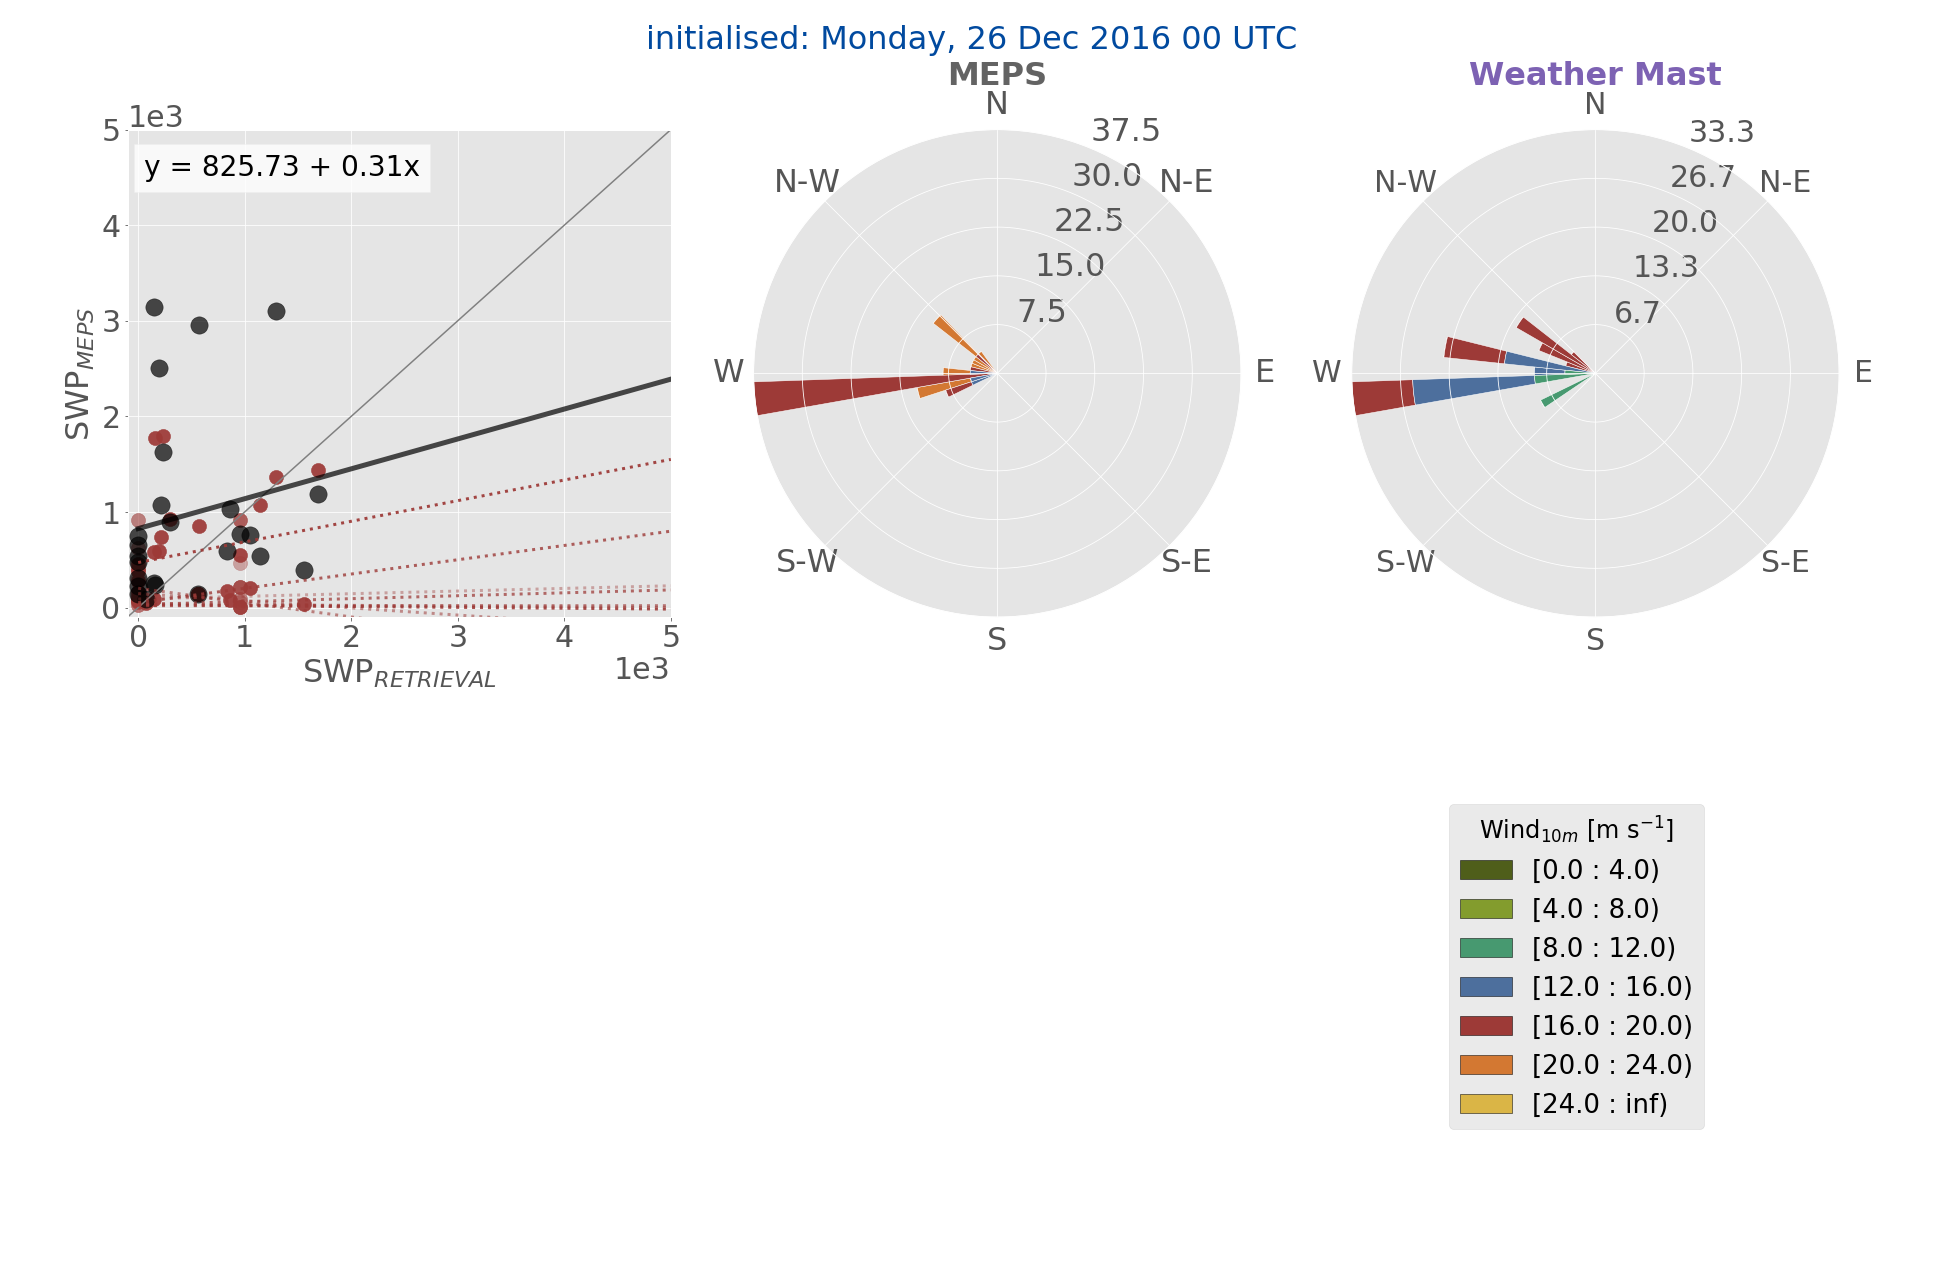
\includegraphics[trim={2.3cm 19.5cm 2.cm .7cm},clip,width=\textwidth]{./fig_windrose/20161226}
		\caption{}\label{fig:wind26}
	\end{subfigure}
	% 	\begin{subfigure}[b]{0.15\textwidth}
	% 		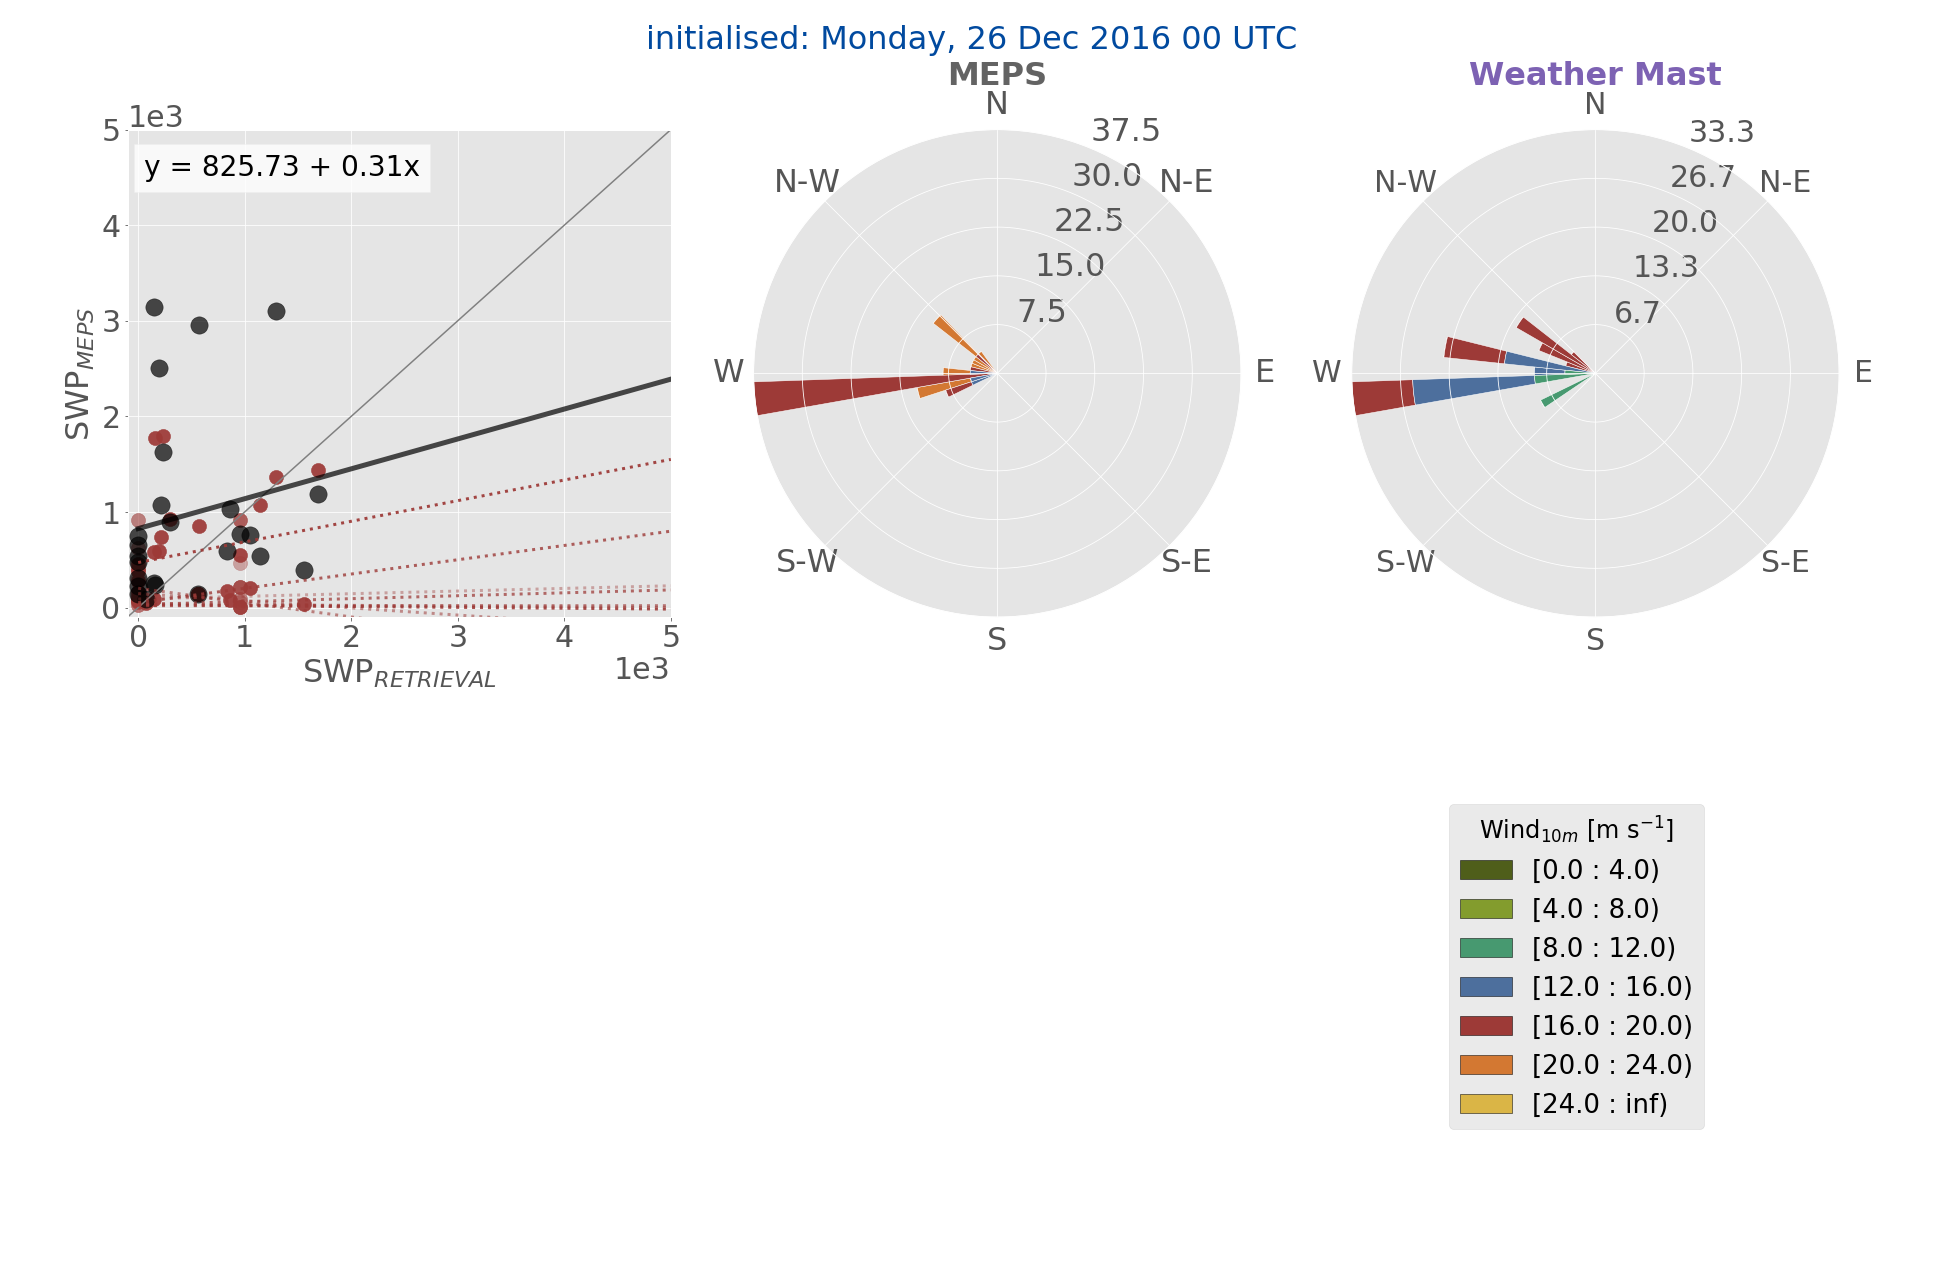
\includegraphics[trim={50.cm 0.cm 8.3cm 28.4cm},clip,width=\textwidth]{./fig_windrose/20161226}
	% 	\end{subfigure}
	\caption{Left panel: Scatter plot of SWP from retrieval and the \num{10} ensemble members initialised at \SI{00}{\UTC} as dots. Black dots and respective best fit (black line) indicate the relation between the deterministic forecast and the retrieval. Red dashed line representing the best fit between the SWP values from MEPS (ensemble member \numrange{2}{10}) and the retrieval. 2nd panel: hourly deterministic forecast wind roses from MEPS initialised at \SI{00}{\UTC}. 3rd panel: \SI{10}{\metre} observed wind at the Haukeliseter measurement site, wind speeds according to the colorbar. }\label{fig:SWP_wind}
\end{figure}